% !TeX document-id = {af928648-7a45-486b-aa45-9066bfc9e040}
% !TeX spellcheck = en-US
% !TeX encoding = utf8
% !TeX program = pdflatex
% !BIB program = biber

\let\ifdeutsch\iffalse
\let\ifenglisch\iftrue
\input{pre-documentclass}
\documentclass[
a4paper,
twoside,
% bibliography=totoc,
% dxtotoc,   %Index ins Inhaltsverzeichnis
% liststotoc, %List of X ins Inhaltsverzeichnis, mit liststotocnumbered werden die Abbildungsverzeichnisse nummeriert
headsepline,
cleardoublepage=empty,
parskip=half,
% draft um zu sehen, wo noch nachgebessert werden muss - wichtig, da Bindungskorrektur mit drin
draft=false
]{scrbook}
\input{config}

\usepackage[
title={Evaluation and Integration of an OPC UA Service into a Container-Based Cloud Platform},
author={Viktor Krimstein},
type=bachelor,
institute=iste, % or other institute names - or just a plain string using {Demo\\Demo...}
course={se},
examiner={Prof.\ Dr.\ Stefan Wagner},
supervisor={Dipl.-Ing.\ Wolfgang Fechner,\\Carsten Ellwein,\ M.Sc.},
startdate={November 22, 2017},
enddate={May 22, 2018}
]{scientific-thesis-cover}

\newacronym{api}{API}{Application Programming Interface}
\newacronym{cad}{CAD}{Computer-Aided Design}
\newacronym{cae}{CAE}{Computer-Aided Engineering}
\newacronym{cam}{CAM}{Computer-Aided Manufacturing}
\newacronym{capp}{CAPP}{Computer-Aided Process Planning}
\newacronym{cm}{CM}{Cloud Manufacturing}
\newacronym{cnc}{CNC}{Computer Numerical Control}
\newacronym{com}{COM/DCOM}{Component Object Model/Distributed Component Object Model}
\newacronym{cps}{CPS}{Cyberphysical System}
\newacronym{crm}{CRM}{Customer Relationship Management}
\newacronym{dama}{DAMA}{Design Anywhere, Manufacture Anywhere}
\newacronym{dds}{DDS}{Data Distribution Service}
\newacronym{erp}{ERP}{Enterprise Resource Planning}
\newacronym{hateoas}{HATEOAS}{Hypermedia As The Engine Of Application State}
\newacronym{http}{HTTP}{Hypertext Transfer Protocol}
\newacronym{iaas}{IaaS}{Infrastructure as a Service}
\newacronym{iot}{IoT}{Internet of Things}
\newacronym{isw}{ISW}{Institute for Control Engineering of Machine Tools and Manufacturing Units of the University of Stuttgart}
\newacronym{it}{IT}{Information Technology}
\newacronym{json}{JSON}{JavaScript Object Notation}
\newacronym{m2m}{M2M}{Machine-to-Machine}
\newacronym{mrp}{MRP}{Manufacturing Resource Planning}
\newacronym{nc}{NC}{Numerical Control}
\newacronym{nist}{NIST}{National Institute of Standards and Technology of the United States of America}
\newacronym{nosql}{NoSQL}{Not only SQL}
\newacronym{opc}{OPC}{Open Platform Communications}
\newacronym{opcua}{OPC UA}{Open Platform Communications Unified Architecture}
\newacronym{paas}{PaaS}{Platform as a Service}
\newacronym{plc}{PLC}{Programmable Logic Controller}
\newacronym{poc}{PoC}{Proof of Concept}
\newacronym{qos}{QoS}{Quality of Service}
\newacronym{rest}{REST}{Representational State Transfer}
\newacronym{rnp}{R'n'P}{Rent'n'Produce: Secure Cloud Service for the Commissioning and Control of Production Systems}
\newacronym{saas}{SaaS}{Software as a Service}
\newacronym{soa}{SOA}{Service-Oriented Architecture}
\newacronym{sql}{SQL}{Structured Query Language}
\newacronym{ui}{UI}{User Interface}
\newacronym{url}{URL}{Uniform Resource Locator}
\newacronym{xaas}{XaaS}{Everything is treated as a Service}

\makeindex

\begin{document}
	
	\iftex4ht
	\Configure{$}{\PicMath}{\EndPicMath}{}
	%$
	\Css{body {text-align:justify;}}
	\Configure{graphics*}
	{pdf}
	{\Needs{"convert \csname Gin@base\endcsname.pdf
			\csname Gin@base\endcsname.png"}%
		\Picture[pict]{\csname Gin@base\endcsname.png}%
	}
	\fi
	
	%Tipp von http://goemonx.blogspot.de/2012/01/pdflatex-ligaturen-und-copynpaste.html
	%siehe auch http://tex.stackexchange.com/questions/4397/make-ligatures-in-linux-libertine-copyable-and-searchable
	%
	%ONLY WORKS ON MiKTeX
	%On other systems, download glyphtounicode.tex from http://pdftex.sarovar.org/misc/
	%
	\input glyphtounicode.tex
	\pdfgentounicode=1
	
	%\VerbatimFootnotes %verbatim text in Fußnoten erlauben. Geht normalerweise nicht.
	
	\input{commands}
	\pagenumbering{arabic}
	\Titelblatt
	
	%Eigener Seitenstil fuer die Kurzfassung und das Inhaltsverzeichnis
	\deftripstyle{preamble}{}{}{}{}{}{\pagemark}
	%Doku zu deftripstyle: scrguide.pdf
	\pagestyle{preamble}
	\renewcommand*{\chapterpagestyle}{preamble}
	
	\section*{Abstract}
	
		In the context of Industry 4.0, services are brought to the forefront along with a higher degree of networking. 
		The vision of self-governing systems that exchange information and make decisions without human intervention is a primary goal, but not necessarily the focus of many projects. 
		
		The research project ``Rent'n'Produce: Secure Cloud Service for the Commissioning and Control of Production Systems'' which is currently being processed at the Institute for Control Engineering of Machine Tools and Manufacturing Units of the University of Stuttgart, has the vision of advancing self-directed manufacturing systems. 
		Companies from different industries should be provided with a cloud-based platform that enables a highly flexible production order. 
		
		This bachelor thesis will focus on the integration of a real machine tool into the Rent'n'Produce Cloud Platform by using the Open Platform Communications Unified Architecture. 
		The required functionality of the integrated service should be encapsulated in a virtualization container. 
		This middleware is intended to provide access to configuration and status data of the production resource, to transfer numerical control programs to the machine tool, and to start or stop the part production.
		
	\newpage
	
	\section*{Kurzfassung}
	
		Im Rahmen von Industrie 4.0 werden Services einhergehend mit einem höheren Vernetzungsgrad in den Vordergrund gerückt. 
		Die Vision sich selbst steuernder Systeme, die ohne menschliches Zutun Informationen austauschen und Entscheidungen treffen, ist zwar übergeordnetes Ziel, steht aber nicht unbedingt im Fokus vieler Projekte.
		
		Das Forschungsprojekt \glqq Rent'n'Produce: Sicherer Cloudservice zur Beauftragung und Steuerung von Fertigungssystemen\grqq{} das aktuell am Institut für Steuerungstechnik der Werkzeugmaschinen und Fertigungseinrichtungen der Universität Stuttgart bearbeitet wird, hat die Vision sich selbst steuernder Fertigungssysteme voranzutreiben.
		Unternehmen unterschiedlicher Branchen soll eine cloudbasierte Plattform zu Verfügung gestellt werden, mit der eine hochflexible Fertigungsbeauftragung möglich ist, ebenso wie der administrative Zugriff auf Produktionsressourcen.
		
		Ziel dieser Arbeit ist die Anbindung einer realen Werkzeugmaschine basierend auf der Open Platform Communications Unified Architecture an Rent'n'Produce umzusetzen. 
		Die benötigte Funktionalität der Anbindung soll dabei in einem Virtualisierungscontainer gekapselt werden. 
		Diese Middleware soll den Zugriff auf Konfigurations- und Zustandsdaten der Produktionsressource, die Übertragung von Programmen für numerische Steuerungen auf die Maschine und das Starten wie Stoppen der Bearbeitung ermöglichen.
	
	\cleardoublepage
	
	% BEGIN: Verzeichnisse
	
	\iftex4ht
	\else
	\microtypesetup{protrusion=false}
	\fi
	
	%%%
	% Literaturverzeichnis ins TOC mit aufnehmen, aber nur wenn nichts anderes mehr hilft!
	% \addcontentsline{toc}{chapter}{Literaturverzeichnis}
	%
	% oder zB
	%\addcontentsline{toc}{section}{Abkürzungsverzeichnis}
	%
	%%%
	
	%Produce table of contents
	%
	%In case you have trouble with headings reaching into the page numbers, enable the following three lines.
	%Hint by http://golatex.de/inhaltsverzeichnis-schreibt-ueber-rand-t3106.html
	%
	%\makeatletter
	%\renewcommand{\@pnumwidth}{2em}
	%\makeatother
	%
	\tableofcontents
	
	% Bei einem ungünstigen Seitenumbruch im Inhaltsverzeichnis, kann dieser mit
	% \addtocontents{toc}{\protect\newpage}
	% an der passenden Stelle im Fließtext erzwungen werden.
	
	\listoffigures
	% \listoftables
	
	% Wird nur bei Verwendung von der lstlisting-Umgebung mit dem "caption"-Parameter benoetigt
	% \lstlistoflistings 
	% ansonsten:
	% \ifdeutsch
	% \listof{Listing}{Verzeichnis der Listings}
	% \else
	% \listof{Listing}{List of Listings}
	% \fi
	
	% mittels \newfloat wurde die Algorithmus-Gleitumgebung definiert.
	% Mit folgendem Befehl werden alle floats dieses Typs ausgegeben
	% \ifdeutsch
	% \listof{Algorithmus}{Verzeichnis der Algorithmen}
	% \else
	% \listof{Algorithmus}{List of Algorithms}
	% \fi
	% \listofalgorithms %Ist nur für Algorithmen, die mittels \begin{algorithm} umschlossen werden, nötig
	
	% Abkürzungsverzeichnis
	\printnoidxglossaries
	
	\iftex4ht
	\else
	% Optischen Randausgleich und Grauwertkorrektur wieder aktivieren
	\microtypesetup{protrusion=true}
	\fi
	
	% END: Verzeichnisse
	
	% Headline and footline
	\renewcommand*{\chapterpagestyle}{scrplain}
	\pagestyle{scrheadings}
	\pagestyle{scrheadings}
	\ihead[]{}
	\chead[]{}
	\ohead[]{\headmark}
	\cfoot[]{}
	\ofoot[\usekomafont{pagenumber}\thepage]{\usekomafont{pagenumber}\thepage}
	\ifoot[]{}

	%%%%%%%%%%%%%%%%%%%%%%%%%%%%%%%%%%%%%%%%%%%%%%%%%%%%%%%%%%%%%%%%%%%%%%%%%%%%%%
	%
	% Main content starts here
	%
	%%%%%%%%%%%%%%%%%%%%%%%%%%%%%%%%%%%%%%%%%%%%%%%%%%%%%%%%%%%%%%%%%%%%%%%%%%%%%%
	
	\chapter{Introduction} \label{ch:introduction}
		
		The trend of connecting physical objects with the Internet gave birth to the term \gls{iot}. 
		\gls{iot} envisions applications running with interconnected objects working together to gather data and act in environments by controlling different actuators to enable new functionality with minimal human intervention~\cite{atzori2010internet}.
		With the introduction of \gls{iot} and \gls{cps} concepts in industrial application scenarios, automation is undergoing a tremendous change~\cite{wollschlaeger2017future}.
		By adapting these concepts, the philosophy of ``\gls{dama}'' has emerged in the past decade~\cite{heinrichs2005anywhere,venkatesh2005validating,manenti2011building}. 
		The \gls{dama} approach demands the ability to exchange design and manufacturing data across multiple sites. 
		\gls{dama} also helps establish links between \gls{mrp}, \gls{erp} and \gls{crm}~\cite{xu2012cloud}. 
		
		However, today's networked manufacturing mainly refers to integration of distributed resources for undertaking a single manufacturing task~\cite{li2010cloud}.
		What is lacking in this type of manufacturing regime are the centralized operation management of the services, choice of different operation modes and embedded access of manufacturing equipment and resources, without which a seamless, stable and high quality transaction of manufacturing resource services and a \gls{qos} cannot be guaranteed~\cite{tao2010theory}.
		Further, any attempt to steer processes independently of continuous human interaction requires, in a very wide sense, the flow of information between some kind of sensors, controllers, and actuators ~\cite{sauter2011evolution}.
		
		The vision to drive self-optimizing production systems forward and to manage them through a cloud platform is an important aspect of cloud manufacturing but has not been the focus of many research projects. 
		With the research project \gls{rnp}~\cite{ellwein2016} which is currently being processed at the \gls{isw}, and its available functionalities at the time of writing this thesis, manufacturers of different industries and sectors can use the cloud platform for flexible production assignment and detailed order management. 
		To drive the vision forward, \gls{rnp} aims to integrate features and functionalities to access machine tools directly from the cloud and independently of their physical location and the underlying manufacturing platforms by only relying on a homogeneous \gls{m2m} communication.
		
		Unfortunately, the last requirement is quite a difficult one as manufacturers show a huge heterogeneity in the ways and protocols, the machine tools support for communication and data access~\cite{xu2012cloud}.
		Tackling this challenge two specifications emerged within the last years.
		European manufacturers integrated the \gls{opcua} the extension of its predecessor \gls{opc}, while in the United States \gls{dds} gets more popular~\cite{niggemann2015data}.
		
		\section{Motivation}\label{sec:motivation}
		
			\gls{cm} is a concept which aims to transform the traditional manufacturing process into the cloud and enable users of the platform an intelligent and more comfortable way to manage manufacturing resources and production assignment~\cite{xu2012cloud}. 
			The realization of a shared resource pool, such as shared manufacturing resources and capabilities, and on-demand use of manufacturing services provide users the ability to manage and view resources at any time or place~\cite{tao2011cloud}. 
			It is possible to follow the whole manufacturing process from the designing stage to production and manufacturing companies can scale their production according to the clients' demand~\cite{tao2011cloud}. 
			The motivation of this work is to provide an architectural approach to provision and manage machine tools of manufacturers remotely and to transfer production data down to the machines using an \gls{m2m} standard communication protocol.
			
			In the scope of this work, production data will be represented in form of G-Code.
			G-Code is the term for a programming language that is used to control automated machine tools~\cite{shin2007reincarnation}. 
			It is a industry standard and often referred to as ISO-6983. 
			Each line of G-Code is executed sequentially and contains information for the machine tool on how to perform a specific task.
			
			By integrating this architecture to \gls{rnp} clients would be given the possibility to track, manage and control their machine tools remotely over a cloud platform independent of their local automation infrastructure.
		
		\section{Goals}\label{sec:goals}
			
			The goal of this thesis is to model the integration of a real machine tool into the \gls{rnp} cloud platform by using \gls{opcua}.
			Therefore, use-cases will be researched and evaluated to create an architecture, modeling the specified requirements.
			This architecture will be later on tested, using a prototypical implementation of a \gls{poc}. 
			The required functionality of the integrated \gls{poc} should be encapsulated in a virtualization container. 
			This middleware is intended to provide access to configuration and status data of the production resource, to transfer \gls{nc} programs, generated through a \gls{cad} and \gls{cam} process chain, to the machine tool, and to start or stop the part production. The resulting \gls{poc} should simulate the \gls{cm} processes beginning with the order management and ending with the production of a real part.
			Subgoals are defined as follows:
			
			\begin{itemize}
				
				\item Evaluation and specification of an architecture providing the required functionality.
				
				\item Implementing and integrating a \gls{poc} service based on the developed architecture.
				
				\item The \gls{poc} should be able to store G-Code for the production part description.
				
				\item The \gls{poc} should provide its functionality using  an \gls{api}.
				
				\item Integration of a real milling machine to the \gls{rnp} platform using the \gls{poc}.
				
			\end{itemize}
			
	\newpage
			
		\section{Structure}
		
			This thesis is structured as follows: In \Cref{ch:foundations}, we describe in detail the scope and the research field of this work. 
			Furthermore we provide relations to the \gls{rnp} research project and to the field of \gls{cm}.
			References to the current state of the art are presented in \Cref{ch:state_of_the_art}.
			Afterwards we take a differentiated view on the present state of the research in \Cref{ch:state_of_the_Science}.
			Concepts and methodologies of the \gls{poc} to be developed as part this work are discussed in more detail in \Cref{ch:concept}.
			In \Cref{ch:discusion} we discuss the results of the \gls{poc} implementation.
			\Cref{ch:conclusion_and_outlook} concludes the paper and outlines possible future work.
	
	\chapter{Foundations}\label{ch:foundations}
	
		In \Cref{ch:introduction} we gave a short summary on \gls{cm} and especially of the challenges in terms of \gls{m2m} communication and the current topology at manufacturing sites.
		A motivation, why the integration of new features is beneficial for the research state of \gls{rnp}. 
		To better understand the used terms and suggested concepts, this chapter introduces fundamental knowledge, which is related to this work.
		
		A closer description of the reseach project \gls{rnp} is provided in \Cref{sec:rent_n_produce}.
		The underlying concepts of cloud computing are highlited in \Cref{sec:cloud_computing}.
		Its' applications to manufacturing models are provided in \Cref{sec:cloud_manufacturing} including the \gls{cad}-\gls{cam} process chain.
		\Cref{sec:opc_ua} gives an introduction to the \gls{m2m} communcation protocol used in this work.
		A general overview of the current state of software used in the manufacturing environment is provided in \Cref{sec:software_in_the_production_environment}.
	
		\section{Rent'n'Produce}\label{sec:rent_n_produce}
		
			The research project \gls{rnp} of the \gls{isw} draws on the existing infrastructure and networking in manufacturing companies and relies on a cloud-based platform for the commissioning of machine-tools and equipment~\cite{xen.17b}. The declared goal of the research project is a highly flexible, location-independent production order across company boundaries. The production parts' description required for commissioning can be present in the form of \gls{cad} data or \gls{nc} programs and transmitted to the system by the client. 
			The provided functionality of the \gls{rnp} platform at the beginning of this work is as show in \Cref{fig:rnp_workflow}.
			
			\begin{figure}[htbp]
				\centering
				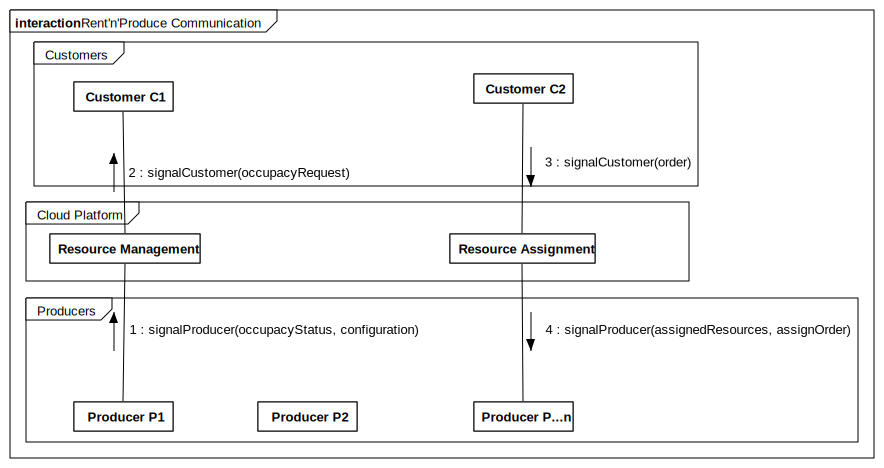
\includegraphics[width=\textwidth]{rnp_workflow.jpg}
				\caption{The workflow of the R'n'P platform.}
				\label{fig:rnp_workflow}
			\end{figure}
			
			Before commissioning the selected resource at the shop floor level, the production part descriptions have to go through a postprocessor and then to be adapted to the selected production resource from the resource catalog.
			This thesis deals with the transfer of existing G-Code data to a production resource. 
			The postprocessing of workpiece descriptions is part of a parallel research project.
			
			\subsection{Initial Architecture}\label{subsec:initial_architecture}
			
			The architecture is based on several services which work independently of each other following a \gls{soa} approach~\cite{erl2008soa}. 
			Each service is split up in a persistence layer and a business logic layer making its functionality accessible to other services using an \gls{api}.
			A simplified view on the architecture of \gls{rnp} is shown in \Cref{fig:rnp_architecture}.
			
			\begin{figure}[htbp]
				\centering
				\includegraphics[width=\textwidth]{rnp_components_simplified.jpg}
				\caption{Simplified architecture of the Rent'n'Produce platform.}
				\label{fig:rnp_architecture}
			\end{figure}
			
			Further, every service is responsible only for one specific part of the whole platform domain(e.g. order management, user access and permission management etc.). 
			The persistence layer serves as a connection from the business logic layer and the database. 
			The business logic layer contains all functionalities regarding the implemented services. 
			
			Services and databases are encapsulated in virtualization containers to ensure platform independence and the increase of maintainability~\cite{xen.17b}. 
			The web interface component is the application layer which contains the \gls{ui} and the \gls{api} gateway routing all client requests to the appropriate services by its internal \gls{url} representation. 
			
		\section{Cloud Computing}\label{sec:cloud_computing}
		
			Explanation of common cloud computing patterns and currently state of the technology respectively to the manufacturing and Internet of Things Industry.~\cite{mell2011nist}
		
		\section{Cloud Manufacturing}\label{sec:cloud_manufacturing}
		
			Brief introduction to cloud manufacturing. Including the general patterns of Cloud Computing and the use of them in the special calse of Cloud Manufacturing. Brief comparison / introduction to The Internet of Things.
		
		\section{OPC UA} \label{sec:opc_ua}
		
			Introduction to communication protocols in manufacturing. Reference to concurrent products on the market.
			
		\section{Software in the Production Environment}\label{sec:software_in_the_production_environment}
		
			Patterns, Software, Virtualization, Cloud Computing, IoT and else.
		
	\chapter{State of the Art}\label{ch:state_of_the_art}
			
		\section{Spring Boot}\label{subsec:spring_boot}
		
		\section{Docker}\label{sec:docker}
		
		\section{Eclipse Milo}\label{sec:eclipse_milo}
		
		\section{Representional State Transfer}\label{sec:rest}
						
	\chapter{State of the Science} \label{ch:state_of_the_Science}
	
		Show the current stae of the science.
		
		\section{Cloud Manufacturing}\label{sec:industry_4}
		
			Summary over the following papers:
			
			\begin{itemize}
				
				\item Industry 4.0 changes through network~\cite{brettel2014virtualization}
				
				\item Automation~\cite{jazdi2014cyber}
				
				\item Multivendor system challenges~\cite{weyer2015towards}
				
				\item Cloud Computing Security~\cite{subashini2011survey}
				
				\item Security SCADA and production systems~\cite{igure2006security}
				
				\item CM Survey~\cite{he2015state}
				
				\item CM Service Models~\cite{li2010cloud}
				
				\item From Cloud Computing to Cloud Manufacturing~\cite{xu2012cloud}
				
				\item Communication protocolls~\cite{wollschlaeger2017future}
				
				\item Industrial Internet of Things~\cite{jeschke2017industrial}
				
			\end{itemize}
		
		\section{Control Engineering in the Cloud}\label{sec:control_engineering_in_the_cloud}
		
			Describing the current state of Control Engineering and Automation from the Cloud.
			ISW project Picasso and TSN related fields.
		
		\section{Machine-to-Machine Communication}\label{sec:machine_to_machine_communication}
		
			Describe the field of M2M by referencing the purposes of OPC UA and other currently available standards. Papers:
				
	\chapter{Concept} \label{ch:concept}
	
		In this chapter, we will describe our concept for the \gls{poc} to be integrated to \gls{rnp}.
		\Cref{sec:requirements} discusses and list requirements for the infrastructure and architecture of the platform, the technology decisions taken for the \gls{poc} implementation as well as mandatory and optional features. In \Cref{sec:approach} we will highlight the implementation approach of the \gls{poc} highlighting the way we integrated the service into the platform. 
		
		\section{Requirements} \label{sec:requirements}
		
			In this section, we will summarize and give an overview over the requirements, gathered from the analysis of the \gls{rnp} platform and the discussion with the research partners.
		
			\subsection{Infrastructure} \label{subsec:infrastructure}
			
				In \Cref{sec:rent_n_produce} we described, that the \gls{rnp} platform is built upon services following the \gls{soa} approach, where each of the services takes responsibility for one specific domain task.
				Further, every service is seperated into a business logic component serving the \gls{api} for its functionality, and a persistence layer component implemented either as a \gls{sql} or \gls{nosql} database.
				Following this pattern, we deduce that the requirement will be to implement the \gls{poc} as a service, which stores the machine-tool configuration data as well as the G-Code for the production part in a database and serves its \gls{api} over a service layer compoenent.
				Further, both components will be realized using Docker containers.
				The business logic container will register itself to the service discovery component and be routable over the \gls{api} gateway.
			
			\subsection{Architecture} \label{subsec:architecture}
			
				As shown in \Cref{subsec:infrastructure} the \gls{poc} to be realized will be packaged into a Docker container and its functionality will be split up into a persistence layer and a business logic layer.
				As the machine-tool integration represents a part of the resource service process, it doesn't need a \gls{ui} integration, as this part is already implemented in the \gls{rnp} architecture.
				
				More precise -- the \gls{poc} should implement an \gls{api}, which can be requested from the resource service, to trigger the production of the required parts contained in a customer order.
			
			\subsection{Technology} \label{subsec:technology}
			
				A core requirement to the \gls{poc} is the support of the \gls{opcua} protocol.
				Over \gls{opcua} the \gls{poc} should communicate with the machine-tools already registered in the resource service of the platform.
				Second requirement is the filtering and recognition of G-Code data as it will be transfered to the \gls{plc} of the machine-tool.
				For the integration to \gls{rnp}, the service should support the communication of \gls{json} over \gls{http} as well as the interaction with the service discovery server and the \gls{api} gateway.
			
			\subsection{Mandatory Features} \label{subsec:mandatory}
				
				Description of the Mandatory Use Cases.
				
				\begin{figure}[htbp]
					\centering
					\includegraphics[width=\textwidth]{use-cases.jpg}
					\caption{The Use-Case diagram for the Proof-of-Concept.}
					\label{fig:use_cases}
				\end{figure}
				
			\subsection{Optional Use-Cases} \label{subsec:optional}	
				
				Description of the optional Use Cases.
				
		\section{Approach} \label{sec:approach}
		
			Introduction to the approach chapter. Point out the proof of concept idea and that it should verify an Open Source service cloud manufacturing approach for further use.
		
			\subsection{Integration} \label{subsec:integration}
			
				Docker, already available R'n'P Platform, etc.
				
			\subsection{Target Architecture} \label{subsec:target_architecture}
			
				Component Diagram etc.
			
			\subsection{Services} \label{subsec:services}
			
				Service Component Diagram taken by the specification, describing which use-case should be handled by which service.
				
			\subsection{Workflow Concept} \label{subsec:workflow_concept}
			
				Sequence Diagram describing the whole workflow of the service and the platform from producer and consumer view.
				
			\subsection{Machine Tool Integration} \label{subsec:machine_tool_intergation}
			
				Description of evaluated NC and PLC decision. Description should reference the general OPC UA file type and lead, to a generic implementation independant of the underlying control.
				
			\subsection{Security} \label{subsec:security}
			
				Details on the security patterns of cloud computing implemented and the patterns of OPC UA Security used in this work.
				
	\chapter{Discusion} \label{ch:discusion}
	
		Discusion how well the actual implementation meets the defined concept goals.
		
		\section{Integration Results}\label{sec:integration_results}
		
			Description of how well the service could be integrated.
			
		\section{Use-Case Implementation}\label{sec:use_cases_implementation}
		
			Discussion and listing of the use-cases and requirements implemented.
			
		\section{Limitations}\label{sec:limitations}
		
			Disscussion of the limitations and difficulities discovered as part of this work.
		
	\chapter{Conclusion and Outlook} \label{ch:conclusion_and_outlook}
	
		Conclusion and Outlook of the work.
		
	\clearpage
	
	% \printindex
	
	\printbibliography
	
	All links were last followed on \today.
	
	\pagestyle{empty}
	\renewcommand*{\chapterpagestyle}{empty}
	\Versicherung
\end{document}
